
\subsection*{3.5 Mensuration}
Mensuration involves calculating lengths, areas, surface areas, and volumes of various geometric shapes. It is divided into two categories: 2D shapes (plane figures) and 3D shapes (solids).

\textbf{Key Concepts:}

\paragraph{1. Areas and Perimeters of 2D Shapes:}
\begin{itemize}
	\item \textbf{Triangle:}
	\[
	\text{Area} = \frac{1}{2} \times \text{base} \times \text{height}, \quad \text{Perimeter} = a + b + c,
	\]
	where $a, b, c$ are the lengths of the sides.
	\item \textbf{Square:}
	\[
	\text{Area} = \text{side}^2, \quad \text{Perimeter} = 4 \times \text{side}.
	\]
	\item \textbf{Rectangle:}
	\[
	\text{Area} = \text{length} \times \text{breadth}, \quad \text{Perimeter} = 2 \times (\text{length} + \text{breadth}).
	\]
	\item \textbf{Trapezium:}
	\[
	\text{Area} = \frac{1}{2} \times (\text{sum of parallel sides}) \times \text{height}.
	\]
	\item \textbf{Parallelogram:}
	\[
	\text{Area} = \text{base} \times \text{height}, \quad \text{Perimeter} = 2 \times (\text{length} + \text{breadth}).
	\]
	\item \textbf{Circle:}
	\[
	\text{Area} = \pi r^2, \quad \text{Circumference} = 2\pi r,
	\]
	where $r$ is the radius.
	\item \textbf{Circular Segment:}
	\[
	\text{Area of Segment} = \frac{r^2}{2}(\theta - \sin\theta), \quad \text{Arc Length} = r\theta,
	\]
	where $r$ is the radius and $\theta$ is the angle in radians.
\end{itemize}

\paragraph{2. Surface Areas and Volumes of 3D Shapes:}
\begin{itemize}
	\item \textbf{Cube:}
	\[
	\text{Surface Area} = 6a^2, \quad \text{Volume} = a^3,
	\]
	where $a$ is the side length.
	\item \textbf{Cuboid:}
	\[
	\text{Surface Area} = 2(lb + bh + hl), \quad \text{Volume} = l \times b \times h,
	\]
	where $l, b, h$ are the length, breadth, and height.
	\item \textbf{Cylinder:}
	\[
	\text{Curved Surface Area} = 2\pi rh, \quad \text{Total Surface Area} = 2\pi r(h + r), \quad \text{Volume} = \pi r^2h,
	\]
	where $r$ is the radius and $h$ is the height.
	\item \textbf{Cone:}
	\[
	\text{Curved Surface Area} = \pi rl, \quad \text{Total Surface Area} = \pi r(l + r), \quad \text{Volume} = \frac{1}{3}\pi r^2h,
	\]
	where $r$ is the radius, $h$ is the height, and $l$ is the slant height.
	\item \textbf{Sphere:}
	\[
	\text{Surface Area} = 4\pi r^2, \quad \text{Volume} = \frac{4}{3}\pi r^3,
	\]
	where $r$ is the radius.
\end{itemize}

\paragraph{Relation Between Mass, Density, and Volume:}
The relationship is given by:
\[
\text{Density} = \frac{\text{Mass}}{\text{Volume}}, \quad \text{Mass} = \text{Density} \times \text{Volume}.
\]

\textbf{Examples:}

\begin{flushleft}
	\textbf{Example 1: Find the area and perimeter of a rectangle with length 8 cm and breadth 5 cm.}
	
	\vspace{0.5cm}
	\textbf{Solution:}
	\vspace{0.5cm}
	
	Area:
	\[
	\text{Area} = \text{length} \times \text{breadth} = 8 \times 5 = 40 \text{ cm}^2.
	\]
	
	Perimeter:
	\[
	\text{Perimeter} = 2 \times (\text{length} + \text{breadth}) = 2 \times (8 + 5) = 26 \text{ cm}.
	\]
	
	Therefore, the area is $40 \text{ cm}^2$ and the perimeter is $26 \text{ cm}$.
\end{flushleft}

\begin{flushleft}
	\textbf{Example 2: Calculate the volume and total surface area of a sphere with radius 7 cm.}
	
	\vspace{0.5cm}
	\textbf{Solution:}
	\vspace{0.5cm}
	
	Volume:
	\[
	\text{Volume} = \frac{4}{3}\pi r^3 = \frac{4}{3}\pi (7)^3 = \frac{4}{3} \times \pi \times 343 \approx 1436.76 \text{ cm}^3.
	\]
	
	Surface Area:
	\[
	\text{Surface Area} = 4\pi r^2 = 4 \times \pi \times (7)^2 = 4 \times \pi \times 49 \approx 615.75 \text{ cm}^2.
	\]
	
	Therefore, the volume is approximately $1436.76 \text{ cm}^3$ and the surface area is approximately $615.75 \text{ cm}^2$.
\end{flushleft}

\begin{flushleft}
	\textbf{Example 3: Find the mass of a cylindrical object with radius 3 cm, height 10 cm, and density $8 \text{ g/cm}^3$.}
	
	\vspace{0.5cm}
	\textbf{Solution:}
	\vspace{0.5cm}
	
	Volume:
	\[
	\text{Volume} = \pi r^2 h = \pi (3)^2 (10) = 90\pi \approx 282.74 \text{ cm}^3.
	\]
	
	Mass:
	\[
	\text{Mass} = \text{Density} \times \text{Volume} = 8 \times 282.74 = 2261.92 \text{ g}.
	\]
	
	Therefore, the mass is approximately $2261.92 \text{ g}$.
\end{flushleft}

\begin{flushleft}
	\textbf{Example 4: In the diagram below, the radius of the sector of circle center $O$ is $7 \, \text{cm}$ and $\angle MON = 60^\circ$. Find, correct to one decimal place, the area of the shaded portion. (Take $\pi = \frac{22}{7}$).}
	
	\begin{center}
		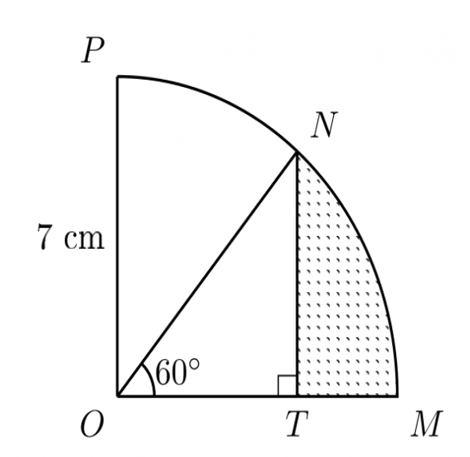
\includegraphics[width=0.6\textwidth]{3.1.png}
		
	\end{center}
	
	\vspace{0.5cm}
	\textbf{Solution:}
	\vspace{0.5cm}
	
	Step 1: Calculate the area of the sector:
	\[
	\text{Area of the sector} = \frac{\theta}{360^\circ} \times \pi r^2.
	\]
	
	Substitute $\theta = 60^\circ$, $r = 7$, and $\pi = \frac{22}{7}$:
	\[
	\text{Area of the sector} = \frac{60}{360} \times \frac{22}{7} \times 7^2.
	\]
	
	Simplify:
	\[
	\text{Area of the sector} = \frac{1}{6} \times \frac{22}{7} \times 49 = \frac{22 \times 49}{42} = \frac{1078}{42} \approx 25.7 \, \text{cm}^2.
	\]
	
	Step 2: Calculate the area of $\triangle OMT$:
	Since $\triangle OMT$ is a right triangle:
	\[
	\text{Area of } \triangle OMT = \frac{1}{2} \times \text{base} \times \text{height}.
	\]
	
	Here, $\text{base} = 7 \, \text{cm}$ and $\text{height} = 7 \, \text{cm}$:
	\[
	\text{Area of } \triangle OMT = \frac{1}{2} \times 7 \times 7 = 24.5 \, \text{cm}^2.
	\]
	
	Step 3: Find the area of the shaded portion:
	\[
	\text{Area of shaded portion} = \text{Area of sector} - \text{Area of } \triangle OMT.
	\]
	
	Substitute:
	\[
	\text{Area of shaded portion} = 25.7 - 24.5 = 1.2 \, \text{cm}^2.
	\]
	
	Therefore, the area of the shaded portion is approximately $1.2 \, \text{cm}^2$.
\end{flushleft}